% SPDX-License-Identifier: LPPL-1.3c
% Copyright (C) 2026 Christophe Jorssen
% Author and Current Maintainer: Christophe Jorssen <christophe.jorssen@gmail.com>
% LPPL maintenance status: maintained
% This file is part of luafemm. See LICENSE and LICENSES.md for its terms.
\section{Alternating fields, eddy currents and skin depth}
\label{sec:harmonic}

\subsection{Diffusion through a conducting slab}
An alternating magnetic field induces currents in a conductor. Their reaction
limits penetration into the material. A planar slab provides a simple case
with an analytical diffusion solution for comparison.

The new ingredient is |frequency|, in hertz. Zero retains the static solver;
a positive value selects the linear single-frequency diffusion problem.
The geometry and material paths remain ordinary TikZ paths. For the slab,
set real, opposite potentials on the two vertical surfaces and natural
conditions on the horizontal surfaces. These boundary conditions describe a slab of finite horizontal thickness,
invariant along the vertical and out-of-page directions.
\begin{codeexample}[code only]
\tikzset{conducting slab/.style={
  femm/problem={frequency=400,xmin=-5,xmax=5,
    ymin=0,ymax=2,mesh size=.25,depth=10},
  femm/boundary={side=all,type=neumann},
  femm/boundary={side=left,type=dirichlet,value=-.0001},
  femm/boundary={side=right,type=dirichlet,value=.0001}},
  femm/materials/slab copper/.style={mu r=1,conductivity=58000000}}
\end{codeexample}
Here the conductivity is $58\,\mathrm{MS/m}$; the key itself expects
$\mathrm{S/m}$. The prescribed vector potentials are in $\mathrm{T\,m}$,
regardless of the millimetre drawing unit. They are phase-zero \emph{peak}
phasors. Register a profile across the slab, then plots the amplitude
of the induced current density:
\begin{codeexample}[code only]
\filldraw[fill=orange!20,
  femm/region={material=slab copper}] (-5,0) rectangle (5,2);
\path[femm/profile={name=skin,samples=101}] (-5,1)--(5,1);
\pic[femm/phase=0,femm/lines=13] {femm field};
% In a PGFPlots axis:
\femmplot[profile=skin,component=Jeddy,abscissa=x,
  representation=amplitude]
\end{codeexample}

For an isotropic conductor, the skin depth is
\[
 \delta=\sqrt{\frac{2}{\omega\mu\sigma}},\qquad \omega=2\pi f.
\]
It is about $3.3043\,\mathrm{mm}$ in this example. Start with a few
triangles per skin depth while adjusting the drawing, then refine the
conductor before trusting the loss estimate. More profile samples do not
resolve the diffusion layer: only a finer \emph{field mesh} does that.
At higher frequency, revisit the local spacing, even if the geometry
has not changed. The automatic mesh has no skin-depth error estimator.

For half-width $a$, surface potential $A_s$ and $k=(1+\mathrm{i})/\delta$,
this slab has $\widehat A(x)=A_s\sinh(kx)/\sinh(ka)$ and
$\widehat J_{\rm eddy}=-\mathrm{i}\omega\sigma\widehat A$.
The following plot compares the finite-element amplitude with this formula
and reports the cycle-average Joule loss for the declared depth.
\luafemmexamplebegin{harmonic-skin}

First prescribe the surface potentials and register the cross-section. The following axis compares its current-density amplitude with the diffusion solution.

% manual example: harmonic-skin/1

\begin{codeexample}[setup code]
\tikzset{conducting slab/.style={femm/problem={frequency=400,
    xmin=-5,xmax=5,ymin=0,ymax=2,mesh size=.25,depth=10},
    femm/boundary={side=all,type=neumann},
    femm/boundary={side=left,type=dirichlet,value=-.0001},
    femm/boundary={side=right,type=dirichlet,value=.0001}},
  femm/materials/slab copper/.style={mu r=1,conductivity=58000000}}
\end{codeexample}

The following picture uses the preceding definitions.

% manual example: harmonic-skin/2

\begin{codeexample}[width=0pt]
\begin{tikzpicture}[conducting slab,scale=3,
    femm/cache={file=\jobname,mode=auto}]
  \filldraw[fill=orange!20,draw=orange!70!black,
    femm/region={material=slab copper}] (-5,0) rectangle (5,2);
  \draw[red,dashed,femm/profile={name=skin,samples=101}] (-5,1)--(5,1);
  \pic[femm/phase=0,femm/lines=13,femm/arrows=false] {femm field};
  \node[above] at (0,2) {$f=400\,\mathrm{Hz}$};
  \femmmeasure[name=skin-loss]
\end{tikzpicture}
\end{codeexample}

% manual example: harmonic-skin/3

\begin{codeexample}[width=0pt]
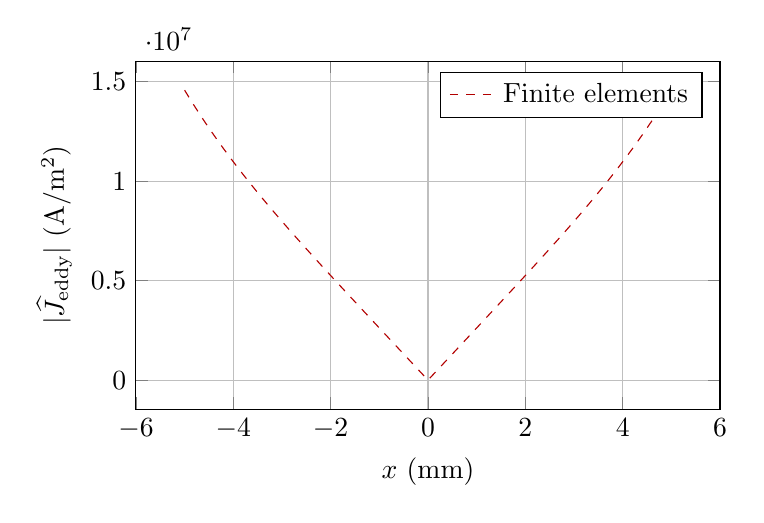
\begin{tikzpicture}
\begin{axis}[width=9cm,height=6cm,grid=major,no markers,
    xlabel={$x$ (mm)},ylabel={$|\widehat J_{\rm eddy}|$ ($\mathrm{A/m^2}$)},
    legend pos=north east]
  \femmplot[profile=skin,component=Jeddy,abscissa=x,
    representation=amplitude,plot options={blue!65!black,thick}]
  \addlegendentry{Finite elements}

  \addplot[red!70!black,dashed,domain=-5:5,samples=101]
    {14576989.91*sqrt((sinh(x/3.304275)^2+sin(deg(x/3.304275))^2)/
      (sinh(5/3.304275)^2+sin(deg(5/3.304275))^2))};
  \addlegendentry{Analytic diffusion solution}
\end{axis}
\end{tikzpicture}
\end{codeexample}

\luafemmexampleend{harmonic-skin}

\subsection{A conducting tube inside the coil}
For an axisymmetric solenoid, a positive frequency works with
|type=axisymmetric|: horizontal coordinates are radii, and all physical volume
integrals include the complete revolution. Add a rectangular copper region
between two positive radii; rotating it produces a conducting tube.

The coil and tube must have different electrical interpretations. The coil
contains insulated fine wires carrying a prescribed terminal current. A named
current-driven series circuit treats its regions as \emph{stranded}: no
resolved eddy current flows through the homogenised winding cross-section.
The tube is a \emph{solid} conductor. Its induced azimuthal currents close around
the axis and react on the coil's field.
\begin{codeexample}[code only]
\tikzset{induction/.style={
  femm/problem={type=axisymmetric,frequency=1000,
    xmax=40,ymin=-40,ymax=40,mesh size=2},
  femm/circuit={name=drive,current=2,phase=0}}}
% In this picture:
\fill[femm/region={material=copper,circuit=drive,
  turns=100,winding fill=.6,mesh size=1}]
  (14,-15) rectangle (18,15);
\fill[femm/region={material=copper,conductor=solid,mesh size=.5}]
  (7,-12) rectangle (10,12);
\end{codeexample}
The default outer boundary still truncates the surrounding air. Refining the
skin layer and enlarging the air domain are separate checks. The complete
example selects the tube for its loss integral and also measures the coil's
complex terminal response.
\luafemmexamplebegin{harmonic-shield}

% manual example: harmonic-shield/1

\begin{codeexample}[setup code]
\tikzset{induction/.style={femm/problem={type=axisymmetric,frequency=1000,
    xmax=40,ymin=-40,ymax=40,mesh size=2},
    femm/circuit={name=drive,current=2,phase=0}},
  femm/materials/solid copper/.style={mu r=1,conductivity=58000000}}
\end{codeexample}

The following picture uses the preceding definitions.

% manual example: harmonic-shield/2

\begin{codeexample}[width=0pt]
\begin{tikzpicture}[induction,scale=.9,
    femm/cache={file=\jobname,mode=auto}]
  \path[femm/region={material=air,mesh size=.6}] (0,-32) rectangle (6,32);
  \filldraw[fill=orange!25,draw=orange!70!black,
    femm/region={material=copper,circuit=drive,turns=100,winding fill=.6,mesh size=1}]
    (14,-15) rectangle (18,15);

  \filldraw[fill=gray!30,draw=gray,
    femm/region={material=solid copper,mesh size=.5}]
    (7,-12) rectangle (10,12);
  \pic[femm/phase=0,femm/lines=17,femm/arrow spacing=14mm] {femm field};
  \draw[red,dashed,femm/profile={name=shield-axis,samples=101}]
    (0,-30)--(0,30);
  \femmselect[name=tube,material=solid copper]
  \femmmeasure[name=tube-loss,selection=tube]
  \femmmeasure[name=drive-terminal,quantity=circuit,circuit=drive]
  \node[above] at (20,40) {$\omega t=0^\circ$};
\end{tikzpicture}
\end{codeexample}

% manual example: harmonic-shield/3

\begin{codeexample}[width=0pt]
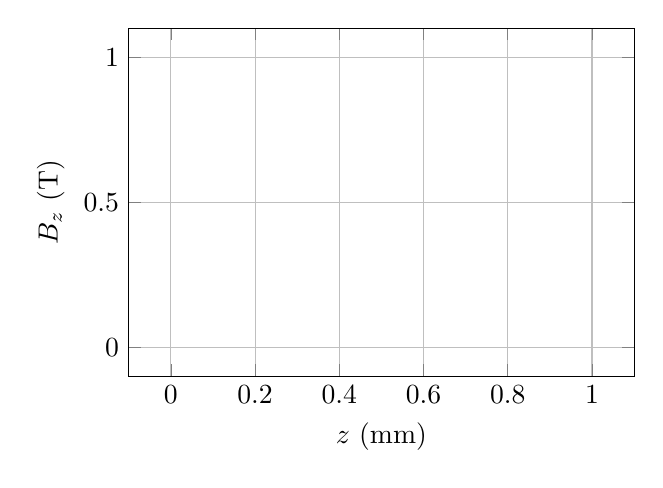
\begin{tikzpicture}
\begin{axis}[width=8cm,height=6cm,grid=major,no markers,
    xlabel={$z$ (mm)},ylabel={$B_z$ (T)},legend style={at={(.5,1.03)},anchor=south}]
  \femmplot[profile=shield-axis,component=Bz,abscissa=z,
    representation=amplitude,plot options={blue!65!black,thick}]
  \addlegendentry{Phasor amplitude}
  \femmplot[profile=shield-axis,component=Bz,abscissa=z,
    representation=snapshot,phase=0,plot options={red!70!black,dashed}]
  \addlegendentry{Instantaneous field at $0^\circ$}
\end{axis}
\end{tikzpicture}
\end{codeexample}

\luafemmexampleend{harmonic-shield}

\subsection{Peak phasors and the meaning of a picture}
Every harmonic source uses the convention
\[
 u(t)=\mathop{\rm Re}\{\widehat u\,e^{\mathrm{i}\omega t}\},\qquad
 \widehat u=u_{\rm re}+\mathrm{i}u_{\rm im}.
\]
A source of amplitude $I$ and phase $\alpha$ therefore has
$\widehat I=I(\cos\alpha+\mathrm{i}\sin\alpha)$. Its instantaneous value at
$\omega t=\theta$ is $I\cos(\theta+\alpha)$.
A negative signed amplitude is allowed; it reverses the source.
Inputs and amplitude plots use peak values, as does FEMM; divide a scalar
phasor amplitude by $\sqrt2$ to obtain its RMS value.
See the \href{https://www.femm.info/doku/doku.php?id=FAQ}{official FEMM FAQ}
for the upstream peak/RMS convention.

A field-line picture is an \emph{instantaneous} snapshot. At phase $\theta$,
it traces contours of $A_{\rm re}\cos\theta-A_{\rm im}\sin\theta$ in planar
mode, or of $2\pi r(A_{\rm re}\cos\theta-A_{\rm im}\sin\theta)$ in axisymmetry.
Arrows follow the corresponding instantaneous vector field. Contours of
$|\widehat A|$ are not substituted for physical field lines. Several pics can
show different phases from the same solution without solving again.
\begin{codeexample}[code only]
\pic[femm/phase=0,femm/lines=17] {femm field};
% An optional second layer, using the same solved phasors:
\pic[femm/phase=90,femm/field style={red,dashed}] {femm field};
\end{codeexample}

\subsection{Keys and order of operations}
Declare the problem, material laws, circuits, boundary conditions and physical
regions first. Register profiles and selections before or after the solve as
usual. A field pic, profile plot or measurement solves on demand. Once meshed,
physical declarations are immutable; create another problem for a frequency
sweep. Drawing phases and plot representations are presentation choices and
do not invalidate the physical cache.

\begin{key}{/femm/problem/frequency=\meta{hertz} (initially 0)}
A finite nonnegative number. Zero selects static magnetics. A positive number
selects the linear complex solver in either planar or axisymmetric geometry.
This is a temporal frequency, independent of spatial winding Fourier orders.
Frequency enters the computation fingerprint; changing it requires a new
solution. A compatible mesh may still be reused. The static |max iterations|
key controls Newton iterations only. Each harmonic field-block GMRES solve has a fixed maximum of
4000 iterations and uses the existing |tolerance| as its relative true-residual
criterion; a failed solve raises an error instead of saving a partial field.
\end{key}

The conductor choices, isolated-current constraints and coupled circuit
sources are documented in Section~\ref{sec:ac-circuits}. By default,
|conductor=auto| selects stranded interpretation for named circuit regions
and solid interpretation otherwise. An unconstrained solid retains the
zero-imposed-voltage model; insulation is not inferred from its geometry.

\begin{key}{/femm/region/current phase=\meta{degrees} (initially 0)}
Phase of the region's signed |current density| amplitude. Only harmonic
problems accept a nonzero phase. For a named winding, use the circuit phase
instead; a nonzero region phase on a circuit leg is rejected. The default
material current density remains a real amplitude unless this key rotates it.
\end{key}

\begin{key}{/femm/circuit/phase=\meta{degrees} (initially 0)}
Phase of the prescribed peak current or voltage, in degrees. Signed turns
still determine each leg's orientation. Series and parallel networks use the
coupled formulation in Section~\ref{sec:ac-circuits}.
\end{key}

\begin{key}{/tikz/femm/phase=\meta{degrees} (initially 0)}
Temporal phase $\omega t$ of a |femm field| pic. It affects both contour geometry
and arrow orientation. It does not modify the stored phasors. Static pictures
ignore temporal phase because their solution is time independent.
\end{key}

\begin{key}{/femm/plot/representation=\meta{choice} (initially snapshot)}
A choice handler accepting |snapshot|, |real|, |imaginary|, |amplitude|, |rms|
and |phase|. It acts on the chosen complex component after projection onto the
profile tangent, normal or polar basis. |phase| returns the principal argument
in degrees in $[-180,180]$; it is not unwrapped, and a zero phasor yields a
plotting gap. |snapshot| returns the instantaneous value at the plot's |phase|.

For the vector norms |B| and |H|, |amplitude| is
$\sqrt{|\widehat u_x|^2+|\widehat u_y|^2}$; |rms| divides this by $\sqrt2$.
The former is the complex vector norm, not in general the maximum instantaneous
length of an elliptically rotating field. |snapshot|, |real| and |imaginary|
return the Euclidean norm of the corresponding real vector. A vector norm has
no unique scalar phase: requesting |representation=phase| with |B| or |H| is
rejected. Choose a signed component instead. Static profiles accept |snapshot|
and |real| only. Harmonic circulation plots are deferred.
\end{key}

\begin{key}{/femm/plot/phase=\meta{degrees} (initially 0)}
Temporal phase for |representation=snapshot|. Other representations ignore
this key. It is independent of the phase selected for field-line pics.
\end{key}

\begin{key}{/femm/plot/component=\meta{component} (initially B)}
Harmonic plots retain the documented magnetic components and add |J| and
|Jeddy|, in $\mathrm{A/m^2}$. These are signed out-of-plane scalar phasors in
planar mode and signed azimuthal scalar phasors in axisymmetry. |J| includes
both impressed and induced currents; |Jeddy| contains only the latter.
For stranded regions |Jeddy=0|. The axisymmetric |flux| component is the full
complex flux $2\pi r\widehat A_\varphi$, in webers.
\end{key}

\subsection{Measurements and power balance}
The existing |\femmselect| and |\femmmeasure| commands retain their syntax.
For |quantity=integrals| on a harmonic model, the available components are
|area|, |volume|, |current_real|, |current_imaginary|, |energy|, |coenergy|,
|joule_loss| and |eddy_loss|. Energy and coenergy are cycle averages and coincide
for the supported real linear permeability. Currents integrate the total
complex current density over the section, without a $2\pi r$ volume factor.
\begin{codeexample}[code only]
\femmselect[name=tube,material=solid copper]
\femmmeasure[name=tube-loss,selection=tube]
\femmvalue[component=joule_loss]{tube-loss}
\end{codeexample}
The reported quantities are
\[
 \overline W=\frac14\int\mathop{\rm Re}
  (\widehat{\mathbf B}\mathbin{\cdot}\widehat{\mathbf H}^{*})\,dV,
 \qquad
 P_{\rm Joule}=\int\frac{|\widehat J|^2}{2\sigma}\,dV.
\]
Nonconducting regions contribute no Joule loss. Stranded regions use the
fill-adjusted conductivity for their prescribed homogenised current.
|eddy_loss| uses only $\widehat J_{\rm eddy}$; it is \emph{not an additive
partition} of |joule_loss| when an impressed current is also present, because
the latter includes an interference term. Use |joule_loss| for heat generation.

For |quantity=circuit|, |current_real|, |current_imaginary| and the available DC
|resistance| are reported. Closed windings additionally provide |linkage_real|
and |linkage_imaginary|. When resistance is known, they provide |voltage_real|,
|voltage_imaginary|, |power|, |reactive_power|, and, at nonzero drive current,
|impedance_real| and |impedance_imaginary|. Units are A, Wb, V, W, var and ohms.
The terminal convention is
\[
 \widehat V=R\widehat I+\mathrm{i}\omega\widehat\lambda,\qquad
 S=\tfrac12\widehat V\widehat I^{*}.
\]
Power is $\mathop{\rm Re}S$ and reactive power is $\mathop{\rm Im}S$.
Mutual coupling is included in linkage: one driven circuit's real power can
include exchange with another source, so it is not automatically a local loss.
No scalar inductance is inferred from this multi-source complex response.
Planar winding closure still requires balanced signed turns per winding;
axisymmetric turns are closed circles. An explicit conductor-length override
changes terminal resistance, while regional loss integrals use the actual
model volume; their sums then need not agree without including the additional
wire volume in the model.

Cycle-average and twice-frequency forces and torques are available through
the interface in Section~\ref{sec:harmonic-force}. Static regional field
averages and scalar |current| are also unavailable for harmonic measurements,
avoiding an implicit choice between a real part and an amplitude.
The low-level real field sampling and section-flux routines retain the
phase-zero snapshot convention. Use phasor profiles for other representations.
For |\femmstat|, harmonic |peak| is the largest centroid complex B-vector norm;
|net_current| and |net_current_imaginary| are the real and imaginary total
section currents. |gmres| is the iteration count; static |newton| and |cg|
statistics are zero.

\subsection{Formulation, validation and current limits}
The unknown is a continuous complex P1 $A_z$ or $A_\varphi$. With $C(v)$ the
appropriate planar or cylindrical curl and real reluctivity tensor $\nu$,
assembly adds the consistent conductive mass to the static stiffness:
\[
 \int \nu C(\widehat A)\mathbin{\cdot}C(v)\,d\Omega
 +\mathrm{i}\omega\int\sigma\widehat A v\,d\Omega
 =\int\widehat J_{\rm src}v\,d\Omega+\hbox{boundary terms}.
\]
Here $d\Omega=dx\,dy$ in planar mode and $r\,dr\,dz$ in axisymmetry; the common
$2\pi$ factor is restored in physical volume observables. Axis regularity
still imposes $A_\varphi=0$. The same quadrature is used for assembly and losses.
The real diffusion stiffness and imaginary mass are solved by restarted GMRES
with complex ILU(0), reorthogonalisation and an explicit true-residual check.
The static conjugate-gradient solver is not used on this non-Hermitian system.

The solver supports real positive linear permeability tensors, finite
nonnegative scalar conductivity, real affine boundary phasors, fine-wire
prescribed series currents and conductive bodies. Automatic static potential
gauges are rejected: supply an anchored boundary. General nonlinear harmonic material
laws, resolved individual strands, circular open boundaries,
reduced-sector analytical sliding gaps and motion-induced currents
remain separate extensions. Permanent-magnet coercivity is rejected here;
compute its DC field separately instead of oscillating a permanent source.
Section~\ref{sec:biased-harmonic} describes the supported small-signal extension
around a captured nonlinear DC bias, including permanent-magnet bias.
Section~\ref{sec:losses} adds linear complex permeability and supported insulated
sheet losses. Section~\ref{sec:harmonic-material-models} adds supported effective
wire laws and a restricted nonlinear fundamental approximation. Unsupported
catalogue loss, lamination and wire models are rejected.

The supported linear harmonic |.fem|/|.ans| subset is described in
Section~\ref{sec:interchange}. Unsupported laws and response records fail
explicitly; ordinary phasors preserve their frequency and both parts. The passive
native cache stores both potential arrays and fingerprints frequency, phase,
conductivity and conductor interpretation; format 24 requires recomputing older
snapshots. It is reusable across all three supported TeX formats.

The harmonic regression checks analytic skin-depth convergence,
phase signs, the low-frequency limit, axis regularity, copper losses, complex
terminal power balance, rejected combinations and cache round trips.
Independent validation meshes and solves passive
AC test fixtures with xfemm, comparing complex A/B/H/J, energy and losses.
That test-only file adapter does not widen the public interchange contract.
The generic format matrix exercises profiles, snapshots and shared frozen
phasors in plain LuaTeX, LuaLaTeX and ConTeXt MkIV.


\subsection{Periodic harmonic cells}
\label{sec:harmonic-periodicity}
Planar paired frontiers use the same |femm/frontier={type=periodic}| and
|femm/pair| keys as static models. A pair imposes
$\widehat A_2=s\widehat A_1$ on \emph{both} phasor parts, with $s=+1$ for
periodicity and $s=-1$ for antiperi\-odicity. Translation and rotation use the
existing pair geometry; unequal subdivisions are synchronised before meshing.
The signed elimination is applied to the real stiffness, complex conductivity
mass, imaginary material tensor and source vectors, then undone when
reconstructing the nodal phasors. It does not introduce an arbitrary complex
Bloch phase. Sources, materials and circuit interpretation must describe the
same physical symmetry as the pair.

The conducting strip below represents a cell that repeats horizontally. Its
top potential is prescribed, its bottom potential is zero, and the paired sides
let the solution remain independent of the artificial cell width. The profile
and field contours come from the same diffusion calculation. The profile retains the P1 elementwise field steps;
more profile samples alone do not refine the physical solution. To use
antiperi\-odicity, set |type=antiperiodic| in the pair and provide excitation
consistent with that different symmetry.

\luafemmexamplebegin{periodic-harmonic}

% manual example: periodic-harmonic/1

\begin{codeexample}[width=0pt]
\begin{tikzpicture}[femm/problem={xmin=0,xmax=20,ymin=0,ymax=12,
    mesh size=.8,depth=5,frequency=200},
    femm/pair={first=left,second=right,shift x=20},
    femm/cache={file=\jobname-cell,mode=auto},scale=2.5]
  \fill[orange!12,femm/region={material=copper}] (0,0) rectangle (20,12);
  \path[femm/frontier={name=left,type=periodic}] (0,0)--(0,12);
  \path[femm/frontier={name=right,type=periodic}] (20,0)--(20,12);
  \path[femm/frontier={name=drive,value=.0001}] (0,12)--(20,12);
  \pic[femm/lines=13,femm/arrows=false,femm/field style={blue!65!black}] {femm field};
  \draw[teal,thick,dashed] (0,0)--(0,12) (20,0)--(20,12);
  \draw[black!70] (0,0)--(20,0) (0,12)--(20,12);
  \draw[orange!80!black,densely dotted,thick,
    femm/profile={name=cell-cut,samples=121}] (10,.1)--(10,11.9);
  \node[font=\small,anchor=south] at (10,12.5) {Periodic conducting cell};
\end{tikzpicture}
\end{codeexample}

% manual example: periodic-harmonic/2

\begin{codeexample}[width=0pt]
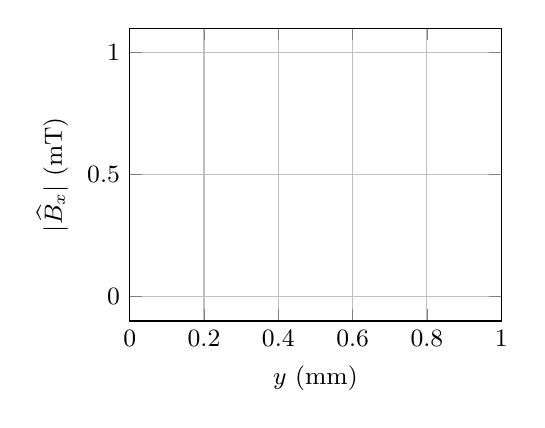
\begin{tikzpicture}
\begin{axis}[width=6.3cm,height=5.3cm,font=\small,xmin=0,xmax=12,grid=major,
    xlabel={$y$ (mm)},ylabel={$|\widehat B_x|$ (mT)},
    y filter/.expression={1000*y},scaled y ticks=false]
  \femmplot[profile=cell-cut,component=Bx,abscissa=y,representation=amplitude,
    plot options={blue!65!black,thick,mark=none}]
\end{axis}
\end{tikzpicture}
\end{codeexample}

\luafemmexampleend{periodic-harmonic}

A harmonic problem that requires an automatic gauge is still rejected; provide
an anchor when the periodic problem has a constant null mode. Antiperiodic
constraints can remove that null mode themselves. Forces are for the actual
modelled selection, with no automatic multiplication by the number of sectors.
Do not use a cut body as if it were a complete closed force contour. The
full-circle moving-band interface does not yet combine with paired sectors,
and analytic AGE interfaces are distinct from this ordinary P1 construction.
Supported harmonic FEM export preserves periodic pairs. Ordinary native AGE
answer import requires an explicit interpolation choice (Section~\ref{sec:native-gaps});
periodic answers without an AGE block remain outside the snapshot importer.
